\documentclass[11pt,a4paper]{article}

\usepackage[utf8]{inputenc}
\usepackage[T1]{fontenc}
\usepackage[english]{babel}
\usepackage{amsmath, amssymb}
\usepackage{geometry}
\usepackage{booktabs}
\usepackage{array}
\usepackage{graphicx}
\usepackage{hyperref}
\usepackage{xcolor}
\usepackage{enumitem}
\usepackage{algorithm}
\usepackage{algpseudocode}
\usepackage{caption}
\usepackage{subcaption}
\usepackage{natbib}

\geometry{margin=2.5cm}
\hypersetup{colorlinks=true, linkcolor=blue, urlcolor=blue, citecolor=blue}

\title{A Linear Benchmark for the Italian Fragility Composite Index\\[0.3em]
  \large Predicting IFC from GRINS Municipal Indicators via LASSO}
\author{Applied Statistics Project}
\date{}

\begin{document}
\maketitle

\begin{abstract}
\noindent
This report documents the construction, validation, and interpretation
of a linear regression benchmark for the raw values of the Italian
Fragility Composite Index (IFC), built from the indicators of the GRINS
municipal panel. The work walks through every analytical choice that
was made and explains why each was preferred over the alternatives that
were tested. Variable selection is carried out with LASSO; the final
deliverable is an ordinary linear model fit on the LASSO-selected
predictors. Performance is assessed by repeated, panel-aware
cross-validation, which prevents the spatial information leakage that
naïve random splits would introduce. The benchmark reaches an
out-of-sample \(R^{2} = 0.825 \pm 0.008\), with a typical absolute
error of \(1.3\) IFC points. A baseline that only knows population and
year explains \(8\%\) of the variance; GRINS adds the remaining
\(74\%\). An ablation experiment attributes most of the predictive
power to careful feature engineering rather than to the regulariser
itself. A core of \(77\) predictors is selected consistently in every
one of the \(25\) cross-validation folds and admits a coherent
substantive interpretation in terms of economic wealth, air quality,
and tourism specialisation. The benchmark is intended as the reference
performance level against which future non-linear models will be
evaluated.
\end{abstract}

\tableofcontents
\vspace{1em}

\section{Introduction and Objective}
\label{sec:intro}

The Italian Fragility Composite Index (IFC) summarises the
multi-dimensional vulnerability of Italian municipalities into a single
numerical score. The index is constructed from a curated list of
indicators with fixed weights, and the source dataset used for this
project reports both the raw IFC values and their decile
classifications. A useful sanity check is that the deciles recomputed
from the raw values match the official deciles of the Municipal
Fragility Index (MFI) for \(95.6\%\) of the municipalities in 2021,
supporting the reliability of the raw IFC values used here as the
modelling target.

The research question we address is to what extent the IFC can be
predicted from an independent collection of municipal indicators (the
GRINS dataset), and which of those indicators carry the most
information. The deliverable is a \emph{linear benchmark}: a model that
is interpretable, fast to fit, and whose performance can serve as a
reference point against which more flexible non-linear models will be
compared in the next phase of the project. The instructor's
specification was a simple linear regression whose predictors are
selected by LASSO; the present report executes that specification and
also documents the supporting analyses that justify the methodological
choices made along the way.

\section{Data}
\label{sec:data}

The target variable is the raw IFC value, drawn from the file
\texttt{IFC\_Final\_Analysis\_Sorted.xlsx}, which reports IFC values
for the years 2019 and 2021 along with their decile classifications and
their agreement with the official MFI decile. The candidate predictors
are taken from the GRINS municipal panel
(\texttt{GRINS\_COMUNALE\_FINAL\_V3.rds}), which contains
\(549\) columns for approximately seven thousand nine hundred
municipalities over the years 2010--2022.

Two GRINS releases were available: an older 110-column version and the
\emph{Final V3} 549-column version. A preliminary run with the smaller
release achieved an out-of-sample \(R^{2} \approx 0.34\), while the
same pipeline on the V3 release achieved \(R^{2} \approx 0.70\). The
V3 release was therefore adopted for all subsequent analyses; the gain
is explained by the much broader coverage of socio-economic
indicators (employment by sector and firm size, taxpayer brackets,
public-employee composition, air quality, frame-SBS aggregates).

We restrict GRINS to the years 2019 and 2021 to match the target. The
two tables are joined on \((\text{PRO\_COM}, \text{year})\) by inner
join, yielding \(15\,790\) municipality--year observations on
\(7\,886\) unique municipalities; six of the \(15\,796\) IFC rows fail
to match a GRINS record and are discarded.

We \emph{pool} the two years in long format rather than fitting two
separate models. The pooling choice is motivated by three reasons.
First, it doubles the effective sample size, stabilising LASSO
selection. Second, the comparison with a separate-year fit (which we
also ran during preliminary work) showed that the leading predictors
and their signs are nearly identical in 2019 and 2021. Third, an
explicit binary indicator \(\text{year2021} \in \{0,1\}\) is added to
the feature matrix, so that any systematic post-pandemic shift in IFC
is absorbed by a single coefficient and does not contaminate the other
estimates.

\section{Why LASSO: The Regulariser Choice}
\label{sec:regulariser}

Before fixing LASSO as the variable-selection device, we tested three
alternative estimators on the engineered feature matrix described in
Section~\ref{sec:fe}: ordinary least squares (OLS), Ridge regression
(\(\ell_{2}\) penalty), and Elastic Net with a grid search on the
mixing parameter \(\alpha \in \{0.1, 0.2, \ldots, 0.9\}\). Their
generic objective is
\begin{equation}
  \hat{\boldsymbol{\beta}}(\lambda,\alpha) \;=\;
  \arg\min_{\boldsymbol{\beta}}
  \left\{
    \tfrac{1}{2n}
    \lVert \mathbf{y} - \mathbf{X}\boldsymbol{\beta} \rVert_{2}^{2}
    + \lambda
    \Bigl[
      \alpha\,\lVert \boldsymbol{\beta} \rVert_{1}
      + (1-\alpha)\,\tfrac{1}{2}\lVert \boldsymbol{\beta} \rVert_{2}^{2}
    \Bigr]
  \right\},
  \label{eq:enet}
\end{equation}
with \(\alpha=1\) giving LASSO \citep{tibshirani1996}, \(\alpha=0\)
giving Ridge \citep{hoerlkennard1970}, and intermediate \(\alpha\)
giving Elastic Net \citep{zouhastie2005}.

Table~\ref{tab:regulariser} summarises out-of-sample performance on a
common train/test split.

\begin{table}[h!]
  \centering
  \begin{tabular}{lcccc}
    \toprule
    Method & \# predictors used & \# non-zero & \(R^{2}\) (test) & RMSE \\
    \midrule
    OLS (no penalty)             & \(326\) & \(326\) & \(0.821\) & \(1.73\) \\
    Ridge \(\lambda_{\min}\)     & \(326\) & \(326\) & \(0.823\) & \(1.72\) \\
    Elastic Net \(\alpha=0.2\)   & \(326\) & \(323\) & \(0.823\) & \(1.72\) \\
    LASSO \(\lambda_{\min}\)     & \(326\) & \(291\) & \(0.824\) & \(1.72\) \\
    LASSO \(\lambda_{\mathrm{1se}}\) & \(326\) & \(239\) & \(0.823\) & \(1.72\) \\
    \bottomrule
  \end{tabular}
  \caption{Comparison of regularisers on the engineered V3 feature
    matrix, single train/test split. Predictive accuracy is essentially
    identical; LASSO is preferred for parsimony.}
  \label{tab:regulariser}
\end{table}

The four regularised methods deliver essentially the same predictive
accuracy. Two considerations break the tie in favour of LASSO. First,
the project specification explicitly requested LASSO as the
variable-selection device. Second, LASSO is the only method among these
that performs \emph{automatic sparse selection}, producing a smaller and
more interpretable model (\(239\) non-zero coefficients out of \(326\),
compared with the full \(326\) for OLS and Ridge). The fact that
unregularised OLS now achieves \(R^{2}\approx 0.82\) (it had exploded
to \(R^{2} = -994\) before feature engineering) is itself an
informative finding: it shows that on the carefully transformed feature
matrix the conditioning is benign enough that the regulariser
\emph{matters mainly for selection}, not for predictive stability.

The Elastic Net grid search returned \(\alpha = 0.2\) as the
cross-validated optimum, very close to Ridge. This indicates that the
predictor groups are mildly correlated but not so correlated that LASSO
selection becomes erratic; this is corroborated by the stability
analysis reported in Section~\ref{sec:stability}.

\section{Variable Classification and Feature Engineering}
\label{sec:fe}

A naïve application of LASSO to the raw GRINS columns produces a model
with both poor interpretability and serious numerical issues, because
the columns are heterogeneous in nature. Some are absolute counts that
scale with municipal size (number of employees, number of taxpayers,
number of deaths), others are already ratios or indices (mobility
indices, annual pollution means, per-capita green space). Pooling them
without distinction lets the size of the municipality dominate every
count column, and produces grossly skewed predictors whose few
extreme values (Rome, Milan) wield disproportionate leverage.

We therefore classify each numeric column into one of five categories
on the basis of its name and apply a class-specific transformation.
\begin{itemize}[leftmargin=2em]
  \item \textbf{Count} -- non-negative size-dependent quantities. We
    first divide by population and then apply \(x\mapsto\log(1+x)\),
    which compresses the long right tail without losing zeros.
  \item \textbf{Count-negative} -- net flows that can take negative
    values (typically migration balances). We apply per-capita
    normalisation only; the logarithm is not defined on negative values.
  \item \textbf{Size} -- population itself and surface area, retained
    as covariates. We apply \(\log(1+x)\) only, since dividing them by
    population is meaningless.
  \item \textbf{Rate} -- variables that are already on a meaningful
    scale (indices, percentages, per-capita means, pollution levels).
    These are left untransformed.
  \item \textbf{Skip} -- ISTAT codes, free-text names, and
    join-artefact columns. These are removed.
\end{itemize}

After this step, the pipeline applies four further operations:
columns with more than twenty percent missing values are dropped (above
this threshold, imputation injects too much fictitious information);
the remaining missing entries are imputed with the column median;
every column is then \emph{winsorised} at its first and ninety-ninth
percentile, which neutralises the leverage of a small number of
extreme municipalities without removing any rows; finally, columns with
zero variance after these operations are discarded.

The resulting feature matrix has \(326\) columns, distributed as
follows: approximately \(280\) counts, \(41\) rates, three size
variables, two net counts, plus the \(\text{year2021}\) dummy.

\section{Estimation}
\label{sec:estimation}

\subsection{LASSO and \(\lambda\) selection}

Given the design matrix
\(\mathbf{X} \in \mathbb{R}^{n \times p}\) and the response vector
\(\mathbf{y} \in \mathbb{R}^{n}\), LASSO solves
\begin{equation}
  \hat{\boldsymbol{\beta}}(\lambda) \;=\;
  \arg\min_{\boldsymbol{\beta}}
  \left\{
    \tfrac{1}{2n}
    \lVert \mathbf{y} - \mathbf{X}\boldsymbol{\beta} \rVert_{2}^{2}
    + \lambda \lVert \boldsymbol{\beta} \rVert_{1}
  \right\}.
  \label{eq:lasso}
\end{equation}
The \(\ell_{1}\) penalty in equation~\eqref{eq:lasso} forces some
coefficients to be exactly zero, achieving simultaneous estimation and
selection. The penalty strength \(\lambda \geq 0\) controls the
trade-off between fit and sparsity; \(\lambda \to 0\) recovers OLS,
while \(\lambda \to \infty\) drives every coefficient to zero.

We search \(\lambda\) on the grid \(10^{k}\) for \(k\) equispaced
between \(-3\) and \(5\) and select the penalty by ten-fold internal
cross-validation. Two standard choices are evaluated.
\begin{itemize}[leftmargin=2em]
  \item \(\lambda_{\min}\) minimises the cross-validated mean squared
    error.
  \item \(\lambda_{\mathrm{1se}}\) is the largest \(\lambda\) whose CV
    error is within one standard error of the minimum. It trades a
    small amount of in-sample fit for a substantially more parsimonious
    solution.
\end{itemize}
The \(\lambda_{\mathrm{1se}}\) rule is the recommended default for
variable-selection contexts \citep{hastieTF2009}: by choosing the
simplest model that is statistically indistinguishable from the best,
it reduces the risk of selecting noise variables that happen to win
the CV by a small margin. On our data
(Sec.~\ref{sec:perf}--\ref{sec:stability}) the two rules give
essentially identical out-of-sample accuracy but
\(\lambda_{\mathrm{1se}}\) uses one third fewer predictors. We adopt
\(\lambda_{\mathrm{1se}}\) for the final benchmark.

\subsection{Honest performance: repeated panel-aware cross-validation}
\label{sec:perf}

A random train-test split would assign different years of the same
municipality to different folds; the model would then be evaluated on
municipalities whose 2019 (or 2021) observation it has already used in
training, inflating the reported \(R^{2}\). We adopt a
\emph{panel-aware} split: every row of a given municipality (both 2019
and 2021) is kept in the same fold. Performance therefore measures
generalisation to genuinely new municipalities.

To estimate the variability of the metrics across splits, we perform
five repetitions of five-fold panel-aware cross-validation, yielding
\(25\) honest test-set evaluations. The full procedure is summarised
in Algorithm~\ref{algo:panelcv}.

\begin{algorithm}[h!]
  \caption{Repeated panel-aware cross-validation for LASSO}
  \label{algo:panelcv}
  \begin{algorithmic}[1]
    \For{repetition \(r = 1, \ldots, 5\)}
      \State Shuffle the list of unique municipalities with seed \(r\)
      \State Partition municipalities into \(5\) equal folds
        \(\mathcal{C}_1, \ldots, \mathcal{C}_5\)
      \For{fold \(k = 1, \ldots, 5\)}
        \State Test rows: all observations of municipalities in
          \(\mathcal{C}_k\)
        \State Train rows: the complement
        \State Choose \(\hat{\lambda}_{\mathrm{1se}}\) by internal
          five-fold CV on the train set
        \State Fit LASSO on the train set with \(\hat{\lambda}_{\mathrm{1se}}\)
        \State Compute RMSE, MAE, \(R^{2}\) on the test set
        \State Record the set of variables with non-zero coefficient
      \EndFor
    \EndFor
    \State Report mean \(\pm\) sd of metrics across the \(25\) folds
    \State Compute, for each variable, the fraction of folds in which
      it was selected (stability)
  \end{algorithmic}
\end{algorithm}

The reported metrics are
\begin{align}
  \mathrm{RMSE} &= \sqrt{\tfrac{1}{n_{\text{te}}}
                 \textstyle\sum_{i \in \text{test}}(y_i - \hat{y}_i)^2}, \\
  \mathrm{MAE}  &= \tfrac{1}{n_{\text{te}}}
                 \textstyle\sum_{i \in \text{test}} |y_i - \hat{y}_i|, \\
  R^{2}         &= 1 - \frac{\sum_{i \in \text{test}}(y_i - \hat{y}_i)^2}
                       {\sum_{i \in \text{test}}(y_i - \bar{y}_{\text{te}})^2},
\end{align}
all computed on the held-out fold and aggregated as mean and standard
deviation across the \(25\) folds.

\subsection{Stability selection}
\label{sec:stability}

To distinguish predictors that are reliably informative from those
selected only by chance in particular splits, we adopt the
\emph{stability selection} framework of
\citet{meinshausenbuhlmann2010}. For every predictor \(j\), the
\emph{selection probability}
\begin{equation}
  \hat{\pi}_{j}
  \;=\;
  \frac{1}{B} \sum_{b=1}^{B}
  \mathbf{1}\!\bigl\{\hat{\beta}_{j}^{(b)} \neq 0\bigr\},
  \qquad B = 25,
  \label{eq:stab}
\end{equation}
estimates the probability that LASSO would assign a non-zero
coefficient to predictor \(j\) on a randomly drawn training set. We
call the \emph{robust core} the set of predictors with
\(\hat{\pi}_{j} = 1\): those selected in every single fold.

\subsection{Final coefficients and standardised effects}

The headline coefficient vector is obtained by refitting LASSO on the
full dataset with \(\lambda_{\mathrm{1se}}\). Because the feature
matrix is on a transformed scale (typically \(\log(1+x/\text{pop})\)
for counts), raw \(\hat{\beta}_{j}\) values are not directly readable
as ``one extra unit of \(x_{j}\) changes IFC by \(\hat{\beta}_{j}\)''.
We therefore report \emph{standardised effects}
\begin{equation}
  \hat{\beta}_{j}^{\,\text{std}}
  \;=\;
  \hat{\beta}_{j} \cdot \mathrm{sd}(X_{j}),
  \label{eq:stdeff}
\end{equation}
which give the expected change in IFC associated with a
one-standard-deviation shift of the engineered variable
\(X_{j}\).

\subsection{Residual diagnostics}

To check the validity of the linear-model assumptions, we refit an
ordinary linear model on the LASSO-selected predictors and inspect
the residuals. We report residual standard deviation, skewness,
excess kurtosis, the Shapiro--Wilk test (on a sample of five
thousand residuals to avoid power inflation), and the Breusch--Pagan
test for homoscedasticity.

\section{Decomposing the Predictive Power: Ablation Study}
\label{sec:ablation}

The headline metric \(R^{2}\approx 0.83\) is the result of three
distinct modelling choices: the use of the rich V3 predictor set, the
class-specific feature engineering of Section~\ref{sec:fe}, and the
panel-aware split for evaluation. To understand which of these choices
matters most, we ran the five models reported in
Table~\ref{tab:ablation}: a trivial baseline that knows only
population and year, two LASSO models on the raw GRINS V3 columns
(with random and panel-aware splits, respectively), and two LASSO
models on the engineered V3 columns (again with random and panel-aware
splits). All four LASSO variants use \(\lambda_{\mathrm{1se}}\).

\begin{table}[h!]
  \centering
  \begin{tabular}{lccc}
    \toprule
    Model & \# predictors & \(R^{2}\) (test) \\
    \midrule
    \(M_{0}\): baseline \(\bigl[\,\log(\mathrm{Pop}) + \text{year}\,\bigr]\) & \(2\)   & \(0.082\) \\
    \(M_{1}\): V3 raw + random split (LASSO.1se) & \(393\) & \(0.700\) \\
    \(M_{2}\): V3 raw + panel split  (LASSO.1se) & \(393\) & \(0.691\) \\
    \(M_{3}\): V3 + FE + random split (LASSO.1se) & \(326\) & \(0.830\) \\
    \(M_{4}\): V3 + FE + panel split  (LASSO.1se) & \(326\) & \(0.824\) \\
    \bottomrule
  \end{tabular}
  \caption{Ablation study. The headline benchmark is \(M_{4}\).}
  \label{tab:ablation}
\end{table}

Reading the table:
\begin{itemize}[leftmargin=2em]
  \item The contribution of GRINS over the trivial baseline is
    \(0.824 - 0.082 = +0.74\) of \(R^{2}\); the bulk of IFC variation
    is socio-economic, not driven by population size.
  \item The effect of feature engineering, at fixed split design, is
    \((M_{4} - M_{2}) = +0.13\) (panel split) and
    \((M_{3} - M_{1}) = +0.13\) (random split). It is by far the
    dominant component of the gain.
  \item The effect of switching from a random split to a panel-aware
    split is \(-0.006\) on the feature-engineered model. This is
    small in absolute terms but it confirms that the headline number
    is \emph{not inflated} by leakage between train and test.
\end{itemize}

The take-away of the ablation is that the bottleneck on this problem
is the \emph{quality of the features}, not the choice of regulariser
or the inferential statistic used to read the residuals.

\section{Results}
\label{sec:results}

\subsection{Predictive performance}

The headline cross-validated metrics, aggregated over \(25\)
panel-aware folds, are reported in Table~\ref{tab:cv}.

\begin{table}[h!]
  \centering
  \begin{tabular}{lcccc}
    \toprule
    Model & \(R^{2}\) (mean \(\pm\) sd) & RMSE & MAE & \# selected \\
    \midrule
    LASSO \(\lambda_{\mathrm{1se}}\) & \(0.825 \pm 0.008\) &
      \(1.74 \pm 0.04\) & \(1.31 \pm 0.02\) & \(163\) \\
    LASSO \(\lambda_{\min}\)         & \(0.827 \pm 0.007\) &
      \(1.74 \pm 0.03\) & \(1.30 \pm 0.02\) & \(245\) \\
    \bottomrule
  \end{tabular}
  \caption{Out-of-fold performance over twenty-five panel-aware folds.
    The two penalty rules are statistically indistinguishable;
    \(\lambda_{\mathrm{1se}}\) is the recommended benchmark.}
  \label{tab:cv}
\end{table}

The standard deviation of \(R^{2}\) across folds is \(0.008\), about
one percent of the mean value: the metric is highly stable across
splits, which is itself evidence of a well-posed estimation problem.

\subsection{Top predictors and substantive reading}

The fifteen predictors with the largest standardised effect on IFC,
ranked by \(\bigl|\hat\beta_{j}^{\,\text{std}}\bigr|\), are listed in
Table~\ref{tab:top15}. All fifteen belong to the
\(77\)-variable robust core. The corresponding bar chart is shown in
Figure~\ref{fig:top15}.

\begin{table}[h!]
  \centering
  \small
  \begin{tabular}{lccc}
    \toprule
    Variable (engineered) & \(\hat\beta\) & \(\mathrm{sd}(X)\) & \(\hat\beta\cdot\mathrm{sd}(X)\) \\
    \midrule
    Total value added per capita (log)               & $-2.74$  & $0.87$ & $-2.38$ \\
    Total employees per capita (log)                 & $+9.53$  & $0.15$ & $+1.45$ \\
    \(\mathrm{PM}_{2.5}\) annual mean                & $-0.27$  & $4.87$ & $-1.30$ \\
    \(\mathrm{PM}_{10}\) annual mean                 & $+0.16$  & $6.35$ & $+1.02$ \\
    Number of local units per capita (log)           & $-39.2$  & $0.02$ & $-0.78$ \\
    Taxpayers in €26k--€55k bracket per capita (log) & $-1.59$  & $0.42$ & $-0.66$ \\
    Services-sector turnover per capita (log)        & $-0.61$  & $1.00$ & $-0.61$ \\
    Total value added per employee                   & $+0.027$ & $17.0$ & $+0.47$ \\
    \(\mathrm{NO}_{2}\) annual mean                  & $+0.071$ & $6.26$ & $+0.45$ \\
    \emph{bonus\_trattamento} per capita (log)       & $-1.71$  & $0.26$ & $-0.45$ \\
    \textbf{year2021}                                & $+0.85$  & $0.50$ & $+0.43$ \\
    Tourism index (beds per inhabitant)              & $+1.15$  & $0.35$ & $+0.40$ \\
    Total establishments per capita (log)            & $-19.7$  & $0.02$ & $-0.40$ \\
    Services-sector employees per capita (log)       & $+1.87$  & $0.20$ & $+0.37$ \\
    High-income share per capita (log)               & $-46.5$  & $0.01$ & $-0.33$ \\
    \bottomrule
  \end{tabular}
  \caption{Top fifteen standardised effects on IFC from the final LASSO
    model. All entries belong to the robust core of seventy-seven
    variables selected in 25/25 cross-validation folds.}
  \label{tab:top15}
\end{table}

\begin{figure}[h!]
  \centering
  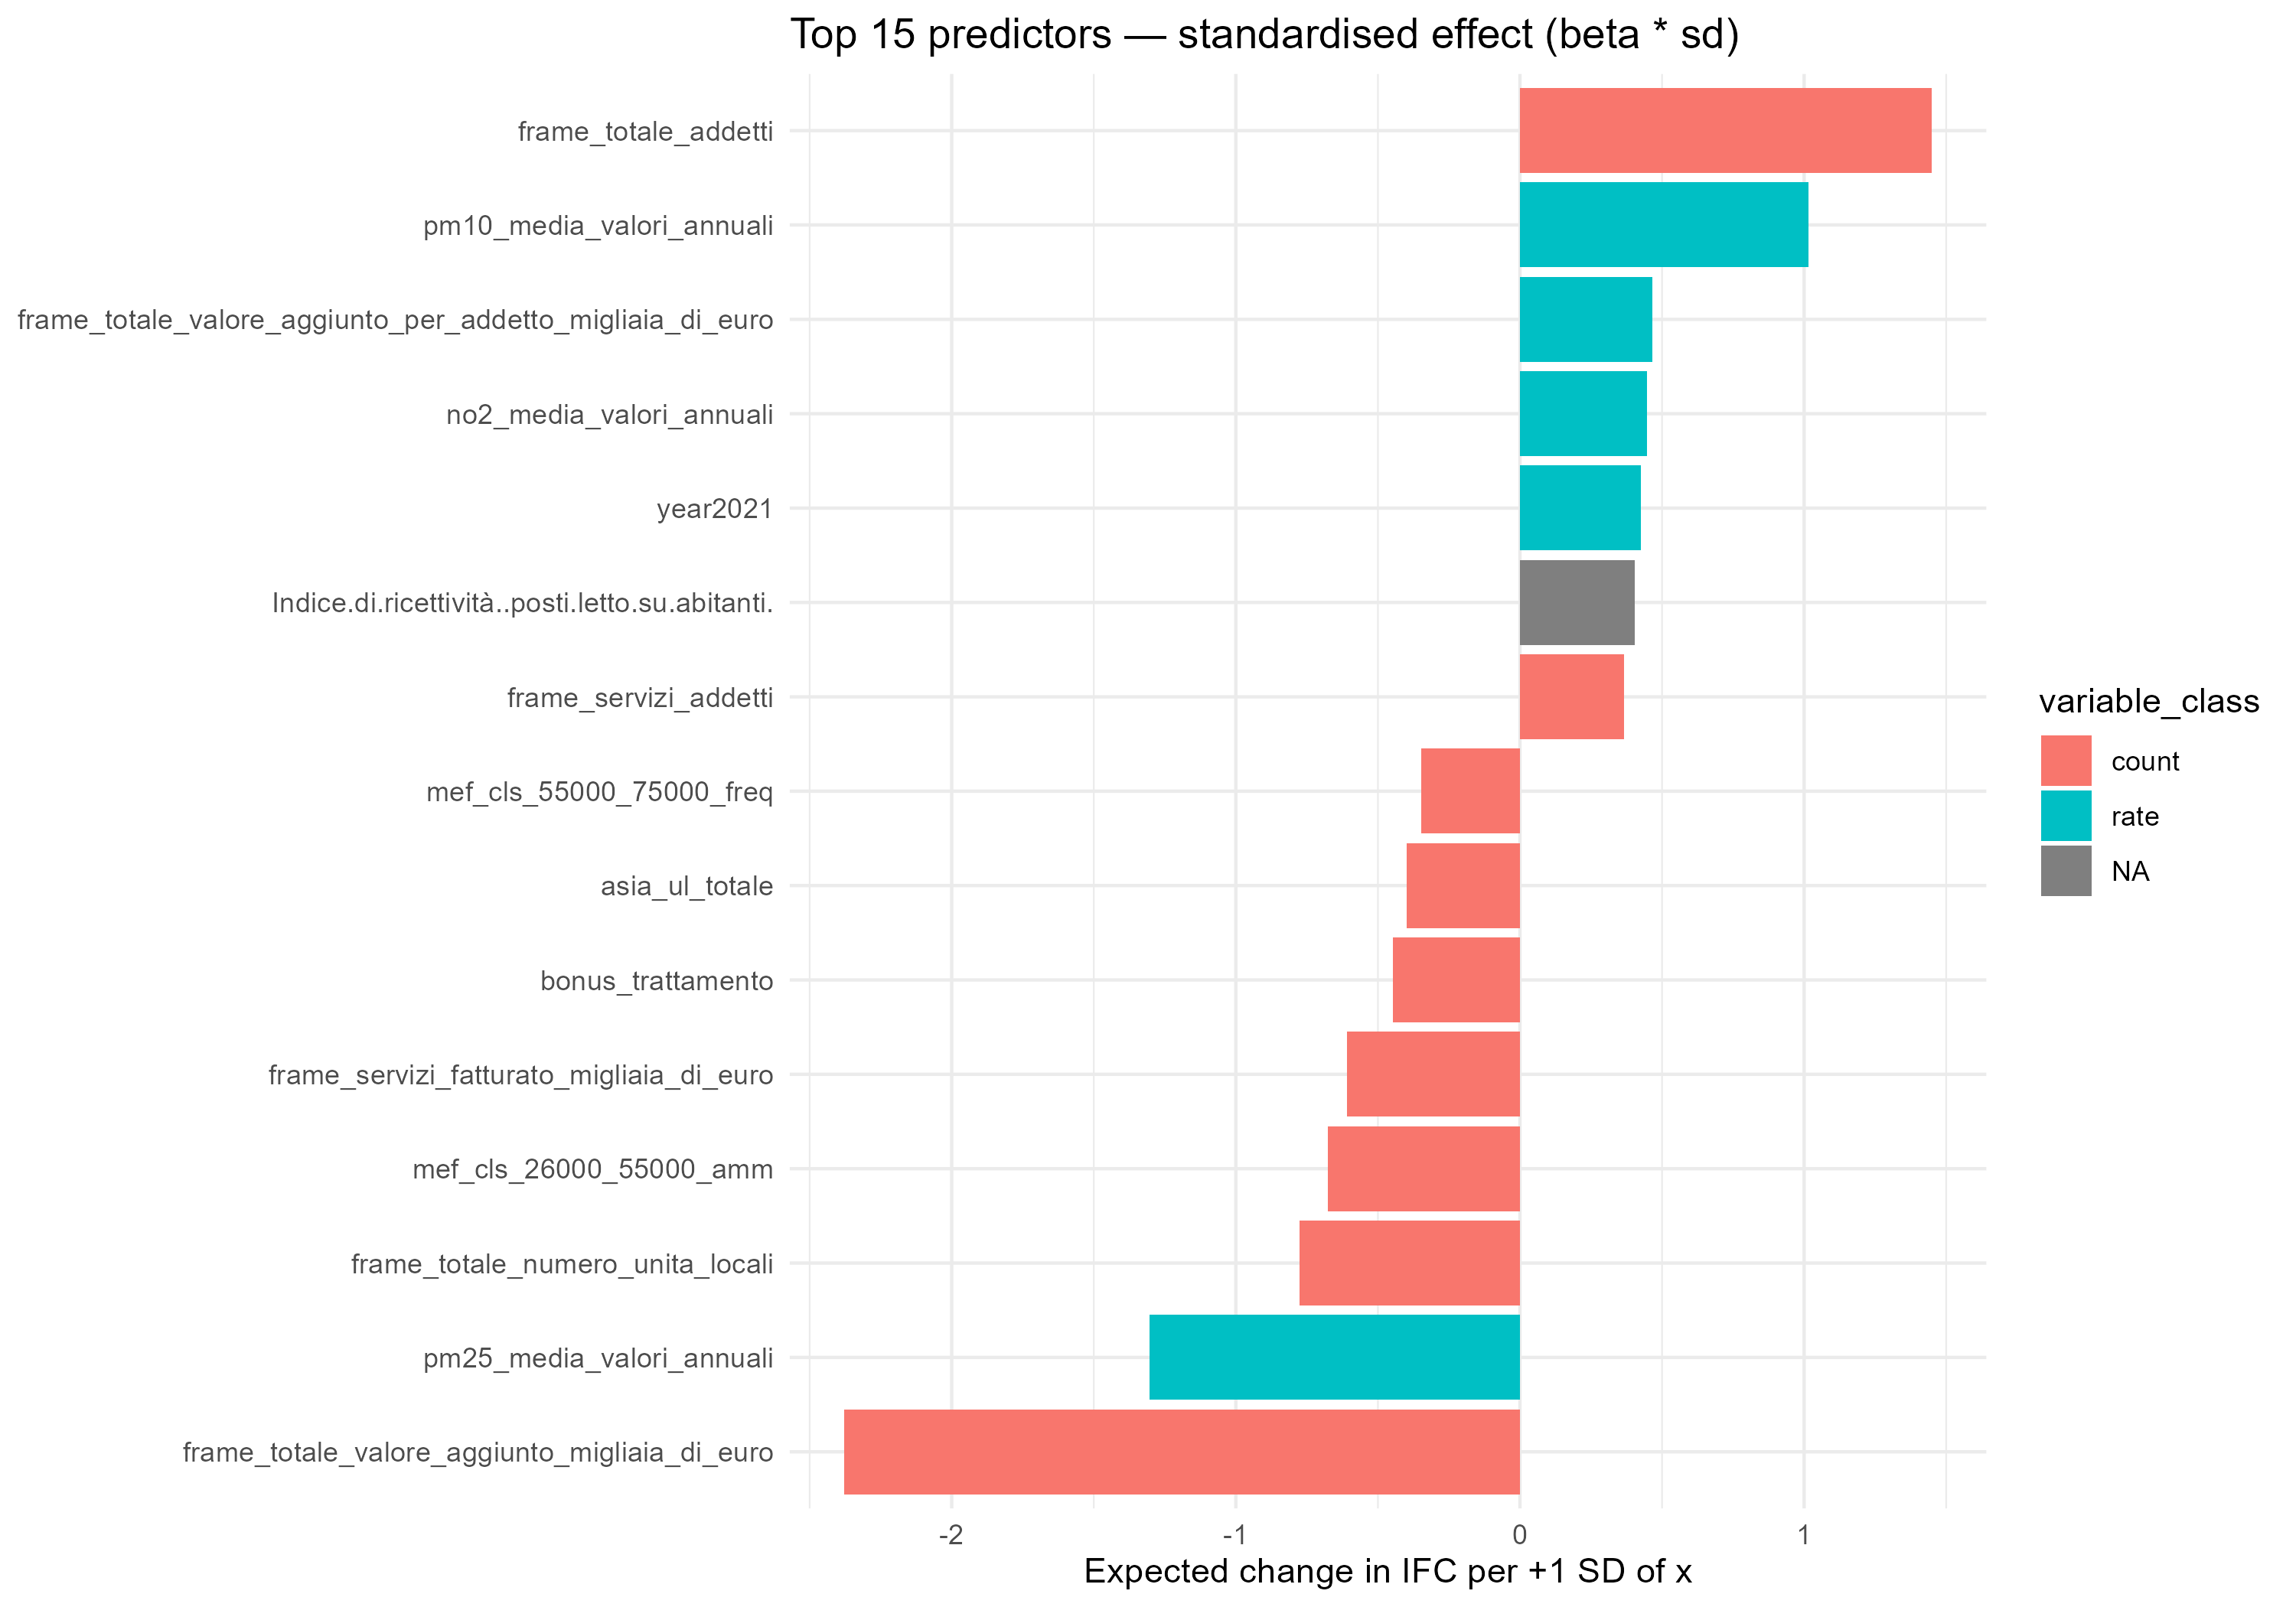
\includegraphics[width=0.85\textwidth]{figures/top15_standardised.png}
  \caption{Top fifteen standardised effects on IFC. Negative bars
    indicate predictors that, when increased, reduce predicted IFC
    (less fragility); positive bars indicate predictors that increase
    it.}
  \label{fig:top15}
\end{figure}

The substantive picture is internally coherent. Wealth-related
indicators (value added per capita, fraction of taxpayers in the mid
income bracket, services-sector turnover, high-income share) carry
negative coefficients: richer municipalities have lower fragility.
Air-quality indicators (\(\mathrm{PM}_{10}\) and \(\mathrm{NO}_{2}\))
enter with positive coefficients, in line with the intuition that
pollution and fragility co-occur. The tourism index enters positively:
municipalities whose economy relies heavily on accommodation services
appear more fragile, consistent with concerns about seasonality and
mono-cultural specialisation. After conditioning on every other
variable, the \(\text{year2021}\) indicator carries a small but clearly
positive coefficient, suggesting a mild post-pandemic worsening of IFC
that is not absorbed by the other GRINS indicators.

\subsection{Stability of the selection}

Out of the \(326\) engineered predictors, \(77\) (about \(24\%\)) are
selected in every one of the \(25\) cross-validation folds and form
the robust core. \(79\) are selected in fewer than \(20\%\) of folds
and behave as noise. The strong bimodality of the selection-frequency
distribution, shown in Figure~\ref{fig:stability}, indicates that the
choice of variables is not driven by the particular split: predictors
either ``always'' or ``almost never'' enter the model.

\begin{figure}[h!]
  \centering
  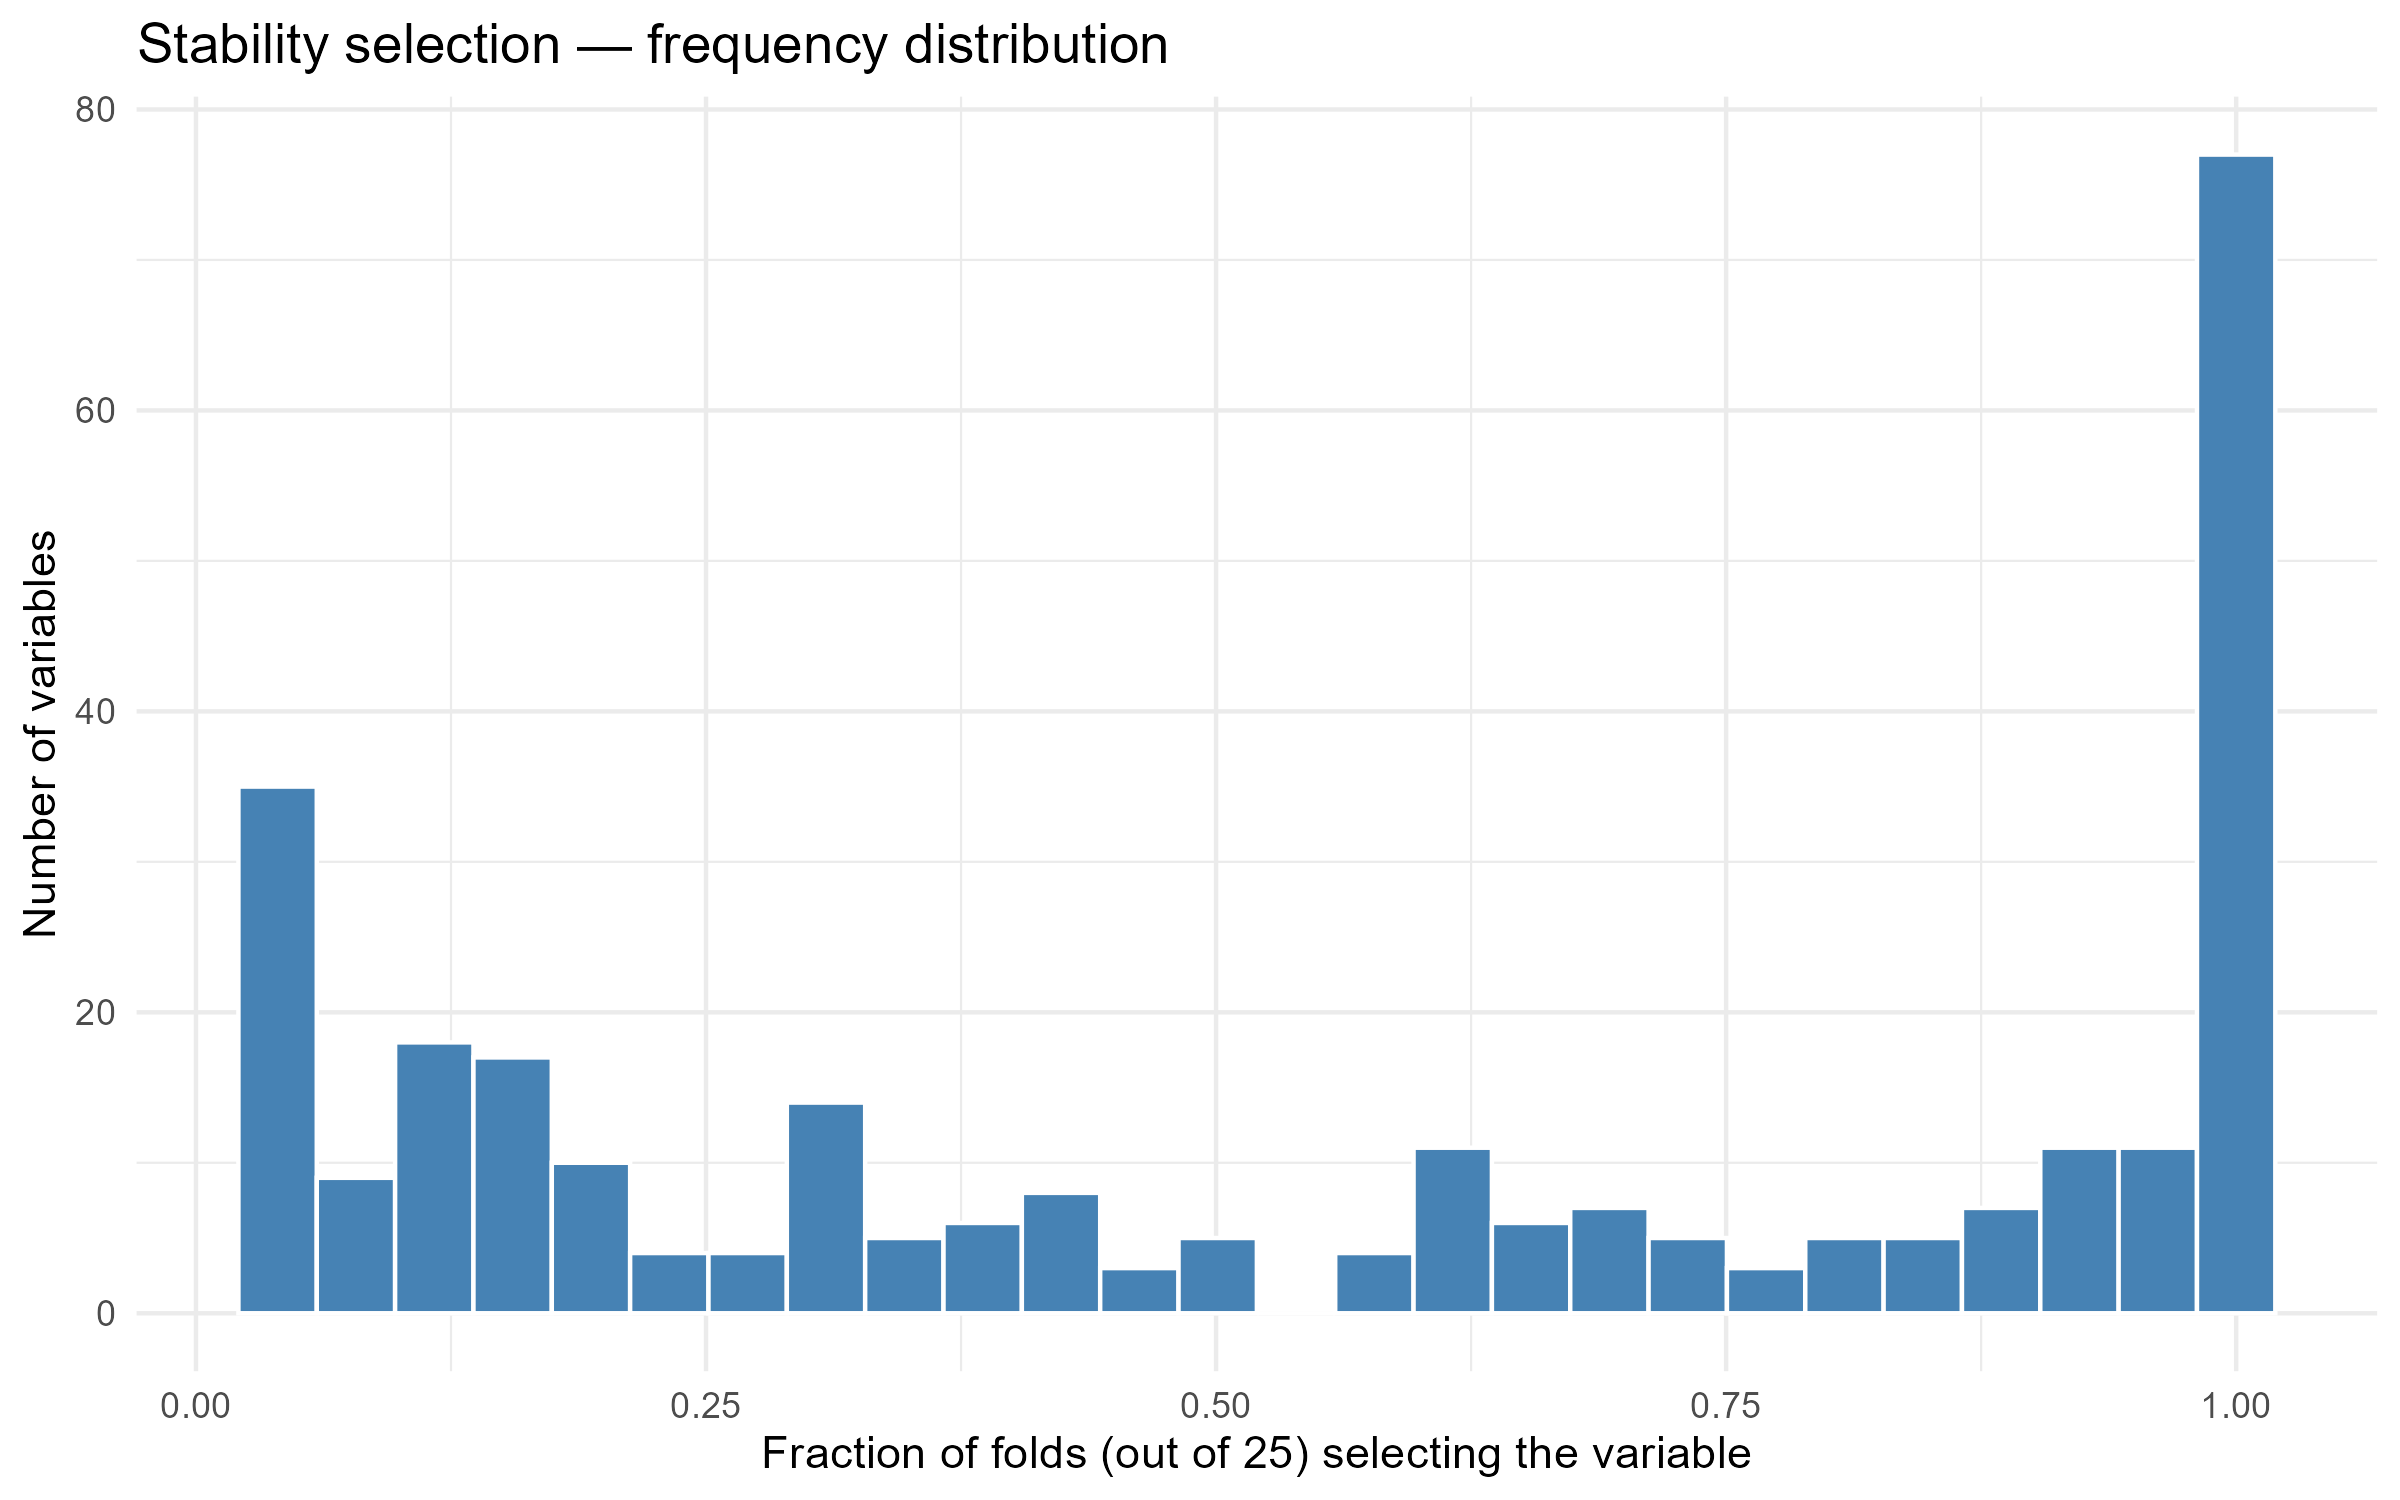
\includegraphics[width=0.75\textwidth]{figures/stability_histogram.png}
  \caption{Stability selection. For each predictor, fraction of the
    twenty-five folds in which LASSO assigned it a non-zero
    coefficient. The mass at the right (frequency~$=1$) is the robust
    core.}
  \label{fig:stability}
\end{figure}

\subsection{Residual diagnostics}

Diagnostics on the OLS refit of the LASSO-selected predictors are
summarised in Table~\ref{tab:diag} and visualised in
Figure~\ref{fig:diag}.

\begin{table}[h!]
  \centering
  \begin{tabular}{lc}
    \toprule
    Diagnostic & Value \\
    \midrule
    Residual standard deviation & \(1.69\) \\
    Skewness                    & \(0.15\) \\
    Excess kurtosis             & \(4.49\) (Normal: \(3.0\)) \\
    Shapiro--Wilk \(p\) (sample of \(5\,000\)) & \(<10^{-22}\) \\
    Breusch--Pagan \(p\)        & \(0.001\) \\
    \bottomrule
  \end{tabular}
  \caption{Residual diagnostics on the OLS refit of the LASSO-selected
    model.}
  \label{tab:diag}
\end{table}

\begin{figure}[h!]
  \centering
  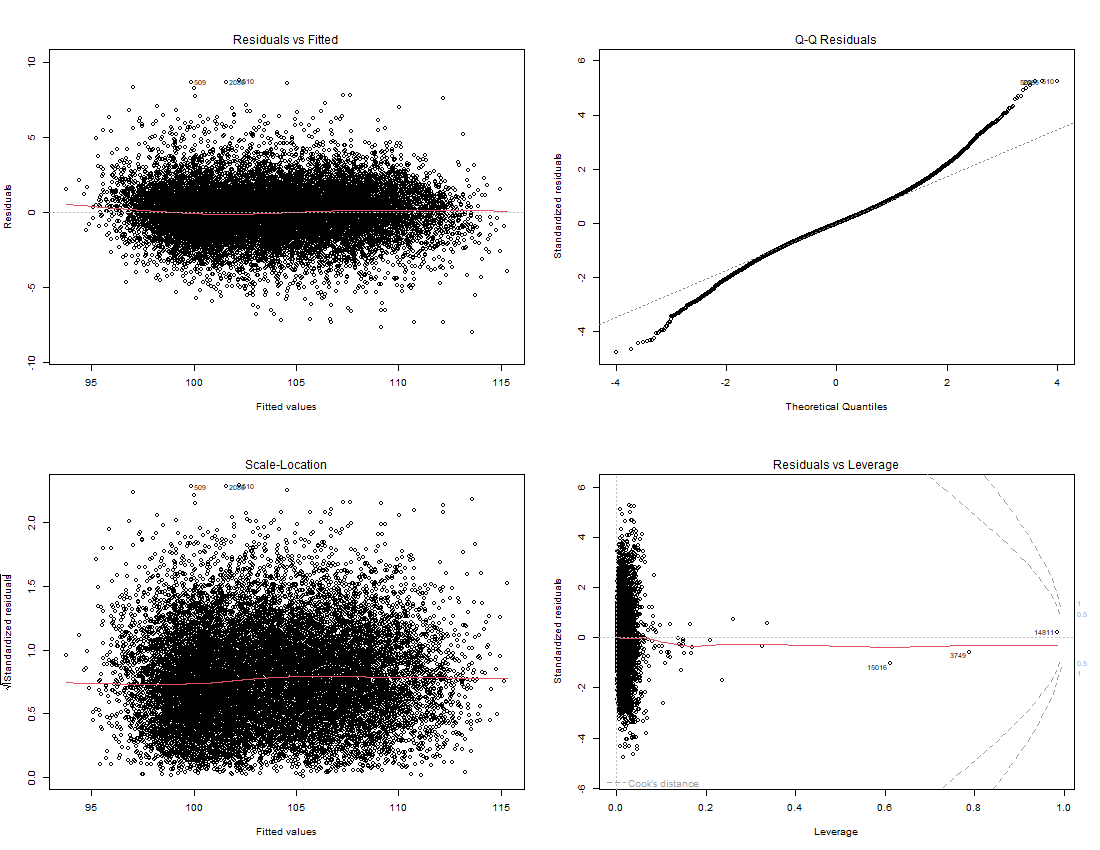
\includegraphics[width=0.9\textwidth]{figures/lm_diagnostics.png}
  \caption{Standard diagnostic plots from the OLS refit on the
    LASSO-selected predictors: residuals against fitted values, normal
    Q--Q plot, scale--location, and residuals against leverage.}
  \label{fig:diag}
\end{figure}

The residual distribution is nearly symmetric (skewness \(0.15\)),
with tails slightly heavier than the Normal (excess kurtosis \(4.5\)
versus the Normal value of \(3.0\)). The Shapiro--Wilk test rejects
normality on a five-thousand-row sample with \(p<10^{-22}\); this is
expected at this sample size, where any minor deviation is flagged as
significant. The Breusch--Pagan test produces \(p=0.001\), evidence
of mild heteroscedasticity. Point predictions remain trustworthy, but
if formal inference on individual \(\hat\beta_{j}\) is required, the
confidence intervals should be computed with
heteroscedasticity-robust standard errors (sandwich, type HC3,
\citealp{long2000}).

\section{Limitations}
\label{sec:limits}

A small number of caveats accompany any use of these results.

First, \(\mathrm{PM}_{10}\) and \(\mathrm{PM}_{2.5}\) have a sample
correlation of \(0.96\); LASSO assigns them opposite signs as a
numerical cancellation, and their individual coefficients should not
be read in isolation. A side experiment that re-fits the model after
dropping each of the two in turn changes the cross-validated MSE by
less than \(3\%\); the \emph{aggregate} pollution effect
(\(\mathrm{PM}_{10}\) and \(\mathrm{NO}_{2}\) together) is, however,
clearly positive and stable across folds.

Second, other clusters of highly correlated variables exist among the
income brackets (\texttt{mef\_cls\_*}) and among the \texttt{frame\_*}
economic-structure columns; within each cluster, the assignment of
magnitude across members is partly arbitrary while the cluster-level
effect is robust.

Third, the positive coefficient of total employees per capita,
conditional on value added per capita being already in the model,
should be read as a residual composition effect rather than a direct
causal statement: holding economic output fixed, additional employees
per capita capture industrial or administrative composition that is
not otherwise accounted for.

Fourth, the mild heteroscedasticity in the residuals suggests that
classical standard errors marginally underestimate uncertainty;
robust standard errors are recommended for formal inference.

Finally, the model is fit on the subset of GRINS columns that survive
the missing-value filter (twenty percent threshold). Indicators with
sparse coverage are therefore not used. A possible refinement is to
adopt more elaborate imputation (multivariate, model-based) but this
goes beyond the scope of the present benchmark.

\section{How the Results Can Be Used}
\label{sec:use}

\paragraph{As a benchmark for future models.}
The principal intended use is to provide a clear performance reference
for non-linear models (generalised additive models, random forests,
gradient boosting machines, neural networks) fit on the same
\((\mathrm{IFC}, \mathrm{GRINS\;V3})\) setup. Any such model should
clear an out-of-sample \(R^{2}\) of approximately \(0.83\) on a
panel-aware split to be worth its additional complexity. A gain of
less than \(0.02\) over the benchmark is unlikely to justify the loss
of interpretability that flexible models typically entail. Conversely,
a substantial gain (say, \(R^{2}\) above \(0.88\)) would indicate that
genuinely non-linear relationships exist in the data and that they
are exploitable.

\paragraph{As an explanatory description of IFC.}
The top predictors with their standardised effects give a substantively
interpretable description of which dimensions drive municipal
fragility: economic wealth and structure pull IFC down, environmental
pollution and tourism specialisation push it up, and a small
post-pandemic worsening is detectable after controlling for everything
else. These dimensions are appropriate anchors for the substantive
narrative of the project.

\paragraph{For imputation and counterfactual analysis.}
Given a new municipality with GRINS measurements, the benchmark
produces an IFC estimate with a typical absolute error of about
\(1.3\) IFC points. The standardised coefficients also support
counterfactual questions of the form ``how much would IFC change if
indicator \(X_{j}\) increased by one standard deviation?'', which is a
policy-relevant exercise.

\paragraph{As a defensible variable shortlist.}
The seventy-seven-variable robust core constitutes a defensible
shortlist for any downstream analysis in which a smaller, more
manageable feature set is preferred (for example, when fitting models
that scale poorly with the number of predictors, or when communicating
results to a non-technical audience).

\paragraph{Reproducibility.}
The full analytical pipeline -- data loading and merging, variable
classification, feature engineering, repeated cross-validation,
LASSO estimation, stability selection, final coefficients, and
diagnostics -- is encapsulated in the script \texttt{final\_benchmark.R}.
With the random seed fixed (\texttt{set.seed(2026)}), rerunning the
script reproduces the headline numbers exactly. The produced output
files (\texttt{repeated\_cv\_summary.csv},
\texttt{final\_coefficients\_standardised.csv},
\texttt{stability\_selection.csv}, and the diagnostic plots)
constitute the technical appendix to this report.

\section{Conclusion}
\label{sec:conclusion}

A linear benchmark for predicting raw IFC values from GRINS municipal
indicators has been established at \(R^{2} = 0.825 \pm 0.008\) on
panel-aware test data, with a typical absolute error of approximately
\(1.3\) IFC points. The GRINS indicators contribute approximately
seventy-four percent of explained variance over a trivial population-
and-year baseline. The ablation study attributes the bulk of the
predictive gain to the class-specific feature engineering of
Section~\ref{sec:fe}: the regulariser matters mainly for parsimony.
The LASSO selection is stable -- a core of seventy-seven predictors is
selected in every one of twenty-five cross-validation folds -- and the
leading predictors admit a coherent substantive interpretation in
terms of economic wealth, air quality, and tourism specialisation. The
model is fit, validated, and interpreted entirely in the \textsf{R}
statistical environment using the \texttt{glmnet} package
\citep{friedman2010glmnet}. The benchmark is now ready to serve as
the reference performance level against which the more flexible
models of the next phase will be evaluated.

\begin{thebibliography}{9}

\bibitem[Friedman et al.(2010)]{friedman2010glmnet}
  Friedman, J., Hastie, T., \& Tibshirani, R. (2010).
  Regularization paths for generalized linear models via coordinate
  descent. \textit{Journal of Statistical Software}, 33(1), 1--22.

\bibitem[Hastie et al.(2009)]{hastieTF2009}
  Hastie, T., Tibshirani, R., \& Friedman, J. (2009).
  \textit{The Elements of Statistical Learning}
  (2nd ed.). Springer.

\bibitem[Hoerl \& Kennard(1970)]{hoerlkennard1970}
  Hoerl, A. E., \& Kennard, R. W. (1970).
  Ridge regression: Biased estimation for nonorthogonal problems.
  \textit{Technometrics}, 12(1), 55--67.

\bibitem[Long \& Ervin(2000)]{long2000}
  Long, J. S., \& Ervin, L. H. (2000).
  Using heteroscedasticity consistent standard errors in the linear
  regression model. \textit{The American Statistician}, 54(3),
  217--224.

\bibitem[Meinshausen \& Bühlmann(2010)]{meinshausenbuhlmann2010}
  Meinshausen, N., \& Bühlmann, P. (2010).
  Stability selection. \textit{Journal of the Royal Statistical
  Society B}, 72(4), 417--473.

\bibitem[Tibshirani(1996)]{tibshirani1996}
  Tibshirani, R. (1996).
  Regression shrinkage and selection via the lasso. \textit{Journal
  of the Royal Statistical Society B}, 58(1), 267--288.

\bibitem[Zou \& Hastie(2005)]{zouhastie2005}
  Zou, H., \& Hastie, T. (2005).
  Regularization and variable selection via the elastic net.
  \textit{Journal of the Royal Statistical Society B}, 67(2),
  301--320.

\end{thebibliography}

\end{document}
